% !TEX program = xelatex
\documentclass[a4paper]{exam}
\usepackage{amsmath}
\usepackage{amsthm}
\usepackage[left=1.8cm,right=1.8cm,top=2.2cm,bottom=2.0cm]{geometry}
\usepackage{ctex}
\usepackage{enumerate}
\usepackage{fancyhdr}
\usepackage{xpatch}
\usepackage{graphicx} 
\usepackage{float} 
\usepackage{subfigure} 
\usepackage{amsfonts}
\usepackage{mathtools}
\usepackage{framed}
\usepackage{multicol}
\usepackage{minted}
\usepackage{hyperref}
\usepackage{tikz}
\usepackage{tabularx}
\usepackage{biblatex}
\addbibresource{09-discussion.bib}
\usetikzlibrary{automata,positioning}
\theoremstyle{definition}
\newtheorem*{solution*}{\textbf{Solution:}}
\newtheorem*{proof*}{\textbf{Proof:}}
\newtheorem{theorem}{Theorem}[subsection]
\newtheorem{definition}{Definition}[subsection]
\newtheorem{lemma}{Lemma}[subsection]
\makeatletter
\newsavebox\mybox
\newsavebox\myboxa
\newsavebox\myboxb
\newsavebox\myboxc
\newsavebox\mybob
\newsavebox\myboc
\newsavebox\myboxd
\newsavebox\myboxe
\newsavebox\myboxf
\newsavebox\mybod
\newsavebox\myboe
\newsavebox\mybof
\newsavebox\myboxg
\newsavebox\mybog
\AtBeginDocument{\xpatchcmd{\@thm}{\thm@headpunct{.}}{\thm@headpunct{}}{}{}}
\makeatother
\printanswers
\pagestyle{fancy}
\renewcommand{\baselinestretch}{1.15}
\usepackage[scaled=0.85]{FiraMono}

\usepackage{paralist}
\let\itemize\compactitem
\let\enditemize\endcompactitem
\let\enumerate\compactenum
\let\endenumerate\endcompactenum
\let\description\compactdesc
\let\enddescription\endcompactdesc

% shorten footnote rule
\xpatchcmd\footnoterule
  {.4\columnwidth}
  {1in}
  {}{\fail}

\title{CS 131 Compilers: Discussion 9: Naive Codegen}
\author{\textbf{杨易为}~~\textbf{吴凌云}~~\textbf{樊雨鑫} \\ \texttt{ \{yangyw,wuly2,fanyx\}@shanghaitech.edu.cn}}


\begin{document}
\begin{lrbox}{\mybox}\begin{minipage}[t]{1.5in}
  \begin{verbatim}
li a0 i
  \end{verbatim}
\end{minipage}\end{lrbox}

\begin{lrbox}{\myboxa}\begin{minipage}[t]{1.5in}
  \begin{verbatim}
cgen(e1)
push $a0
cgen(e2)
$t1 <= top
add $a0 $t1 $a0
pop
  \end{verbatim}
\end{minipage}\end{lrbox}

\begin{lrbox}{\mybob}\begin{minipage}[t]{1in}
 if e1 = e2 then e3 else e4
\end{minipage}\end{lrbox}

\begin{lrbox}{\myboxb}\begin{minipage}[t]{1.5in}
  \begin{verbatim}
cgen(e1)
push $a0
cgen(e2)
$t1 <=top
pop
beq $a0 $t1 true_branch
false_branch:
cgen(e4)
j end_if
true_branch:
cgen(e3)
end_if:
  \end{verbatim}
\end{minipage}\end{lrbox}

\begin{lrbox}{\myboc}\begin{minipage}[t]{1in}
while e1 = e2 loop e3 pool
\end{minipage}\end{lrbox}

\begin{lrbox}{\myboxc}\begin{minipage}[t]{1.5in}
  \begin{verbatim}
predicate:
 cgen(e1)
 push $a0
 cgen(e2)
 $t1 <= top
 pop
 bne $a0 $t1 end_while
 cgen(e3)
 j predicate
end_while:
  \end{verbatim}
\end{minipage}\end{lrbox}
\begin{lrbox}{\mybod}\begin{minipage}[t]{1in}
def f(x1,...,xn) {e}
\end{minipage}\end{lrbox}


\begin{lrbox}{\myboxd}\begin{minipage}[t]{1.5in}
  \begin{verbatim}
f_entry:
 move $fp $sp
 push $ra
 cgen(e)
 $ra <= top
 addiu $sp $sp 4n+8
 lw $fp 0($sp)
 jr $ra
  \end{verbatim}
\end{minipage}\end{lrbox}

\begin{lrbox}{\myboe}\begin{minipage}[t]{1in}
f(e1,...,en)
\end{minipage}\end{lrbox}


\begin{lrbox}{\myboxe}\begin{minipage}[t]{1.5in}
  \begin{verbatim}
push $fp
cgen(en)
push $a0
...
cgen(e1)
push $a0
jal f_entry
  \end{verbatim}
\end{minipage}\end{lrbox}
\begin{lrbox}{\mybof}\begin{minipage}[t]{1in}
let x: T <- e1 in e2
\end{minipage}\end{lrbox}


\begin{lrbox}{\myboxf}\begin{minipage}[t]{1.5in}
  \begin{verbatim}
cgen(e1, n)
push $a0
cgem(e2,n+1)
pop
  \end{verbatim}
\end{minipage}\end{lrbox}
\begin{lrbox}{\mybog}\begin{minipage}[t]{1in}
Temporary var x(whose offset is at ofs)
\end{minipage}\end{lrbox}


\begin{lrbox}{\myboxg}\begin{minipage}[t]{1.5in}
  \begin{verbatim}
lw $a0 - ofs($sp)
  \end{verbatim}
\end{minipage}\end{lrbox}

\maketitle
\section{cgen For Pure Stack Machine\cite{josehu}}
The cgen Function is an abstraction of how a recursive Code Generator is implemented. cgen $(e 1, n)$ means emitting code for expression e1, when the current available temporary offset is $n$. Offsets only serve let / case expressions because they introduce new temporary variables.

Here we consider the generation of MIPS assembly code from AST structures. Each type of nodes on the input AST must have a corresponding implementation of cgen. We use a pure Stack Machine scheme to simplify the ideas, where:
\begin{enumerate}
    \item  Only assuming 1 preserved Register - the Accumulator $\$ a 0$. to store:
\item Result of each operation (including function return value)
\item Self object pointer on method dispatch
\item Invariants: The stack after each cgen will be exactly the same as at the point of entrance
\item The stack is globally preserved, so usually using the memory as stack, and \$sp for the stack pointer
\item Use \$fp for the frame pointer, the boundary of caller's and callee's responsibility
\end{enumerate}
The following is a summary of implementations of recursive cgen function (without considering OOP):
\begin{center}
\begin{tabularx}{\paperwidth}{|p{1in}|p{1.5in}|p{1in}|p{1.5in}|}
\hline Expression & Implementation & Expression & Implementation\\
\hline Integer i & \usebox\mybox &  e1 + e2  & \usebox\myboxa\\
\hline \usebox\mybob & \usebox\myboxb & \usebox\myboc  & \usebox\myboxc\\
\hline \usebox\mybod & \usebox\myboxd & \usebox\myboe  & \usebox\myboxe\\
\hline \usebox\mybof & \usebox\myboxf & \usebox\mybog  & \usebox\myboxg\\
\hline
\end{tabularx}
\end{center}
The offset $n$ passed down the cgen Function is used at let / case expressions, since they introduce new variables, and we need to save their values in inner scopes.
\subsection{Register Allocation}
Pure Stack Machines are simple but very inefficient. The most direct optimization is to use as much preserved registers ( \$s0 - \$s6 for MIPS) instead of always pushing onto stack. We need the following concepts for analyzing register allocation:

\begin{enumerate}
    \item  Next-Use tells when will the value of $x$ assigned at $x \leftarrow y+z(i)$ be next used.
    \begin{enumerate}
        \item $\circ=j$ if the next closest usage is at $a$ op $x(j)$.
    \end{enumerate}
\item $x$ is Live at some location when:
\begin{enumerate}
    \item  It has been assigned a value previously
\item It will be used after
\item NO interleaving assignment to $x$ between current location and the next usage
\end{enumerate}
\end{enumerate}
\subsection{Determine liveness}
To determine the Liveness of variables in every location inside a Basic B.
\begin{minted}[mathescape,linenos]{c}
void computeLiveness(setlive_at_exit) {
 live_set=live_at_exit;
 for (each instruction i from end to start) {
  /* Suppose i is x <- y op z here. */
  live_set=live_set- {x};
  live_set=Union of live_set and {y, z};
  Liveness at location just before instruction i is live_set;  
 }
}
\end{minted}
To determine the Liveness of variables through out the Data Flow (i.e. across Basic Blocks), we should apply Dataflow Analysis framework, which will be covered in the last chapter.
\section{Register Interference Graph}
After determining Liveness of all variables, we can decide which register should be assigned to which variable. Basic idea is when two Temporaries a,b will live simultaneously at some point, called  interferes with , then they cannot share the same register.
\begin{figure}[htbp]
  \centering
  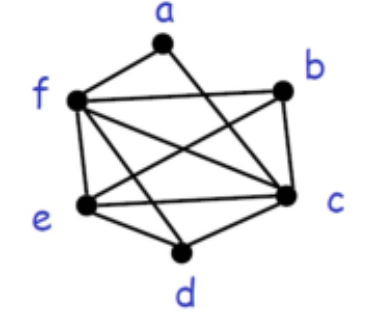
\includegraphics[width=4cm]{./img/reg.png}
\end{figure}
\begin{enumerate}
    \item Each node is a Temporary variable
\item Each edge means an interference between nodes, and that these two nodes cannot share the same register
\end{enumerate}

Finding a solution is a Graph -Coloring problem, which is NP-Hard. We use the following heuristic algorithm to partiallysolve this problem:
\begin{minted}[mathescape,linenos]{python}
dictassignRegister(Graph RIG, set regs) {
  while (RIG is not empty) {
    if (there is a node n with < k neighbors)
     Pushnontostack;
    else {  
      /* Run in short of registers. */
      Pick a victim node n;
      Spill n into memory; 
    }
    Remove n from RIG;  
  }
  for (each node n on stack) {
    Pick a reg $rx from regs, which cannot be already used by one of n's neighbors;
    Assign $rx to n;   
  }
}
\end{minted}
For a victim x spilled into memory, we need:
\begin{enumerate}
    \item load  x every time before using
    \item store x every time after assignment
\end{enumerate}

There may be register pressure
\begin{enumerate}
    \item Some optimizations increase live-ranges:

\begin{enumerate}
    \item Copy propagation
    \item Common sub-expression elimination
    \item Loop invariant removal
\end{enumerate} 
\item In turn, that can cause the allocator to spill
\item Copy propagation isn't that useful anyway:
\begin{enumerate}
 \item Let register allocater figure out if it can assign the same register to two temps!
 \item Then the copy can go away.
 \item And we don't have to worry about register pressure.
 \end{enumerate} 
\end{enumerate}
\section{Coloring with coalescing\cite{cs153lec21}}
To resolve the problem, we use Coalescing Register Allocation.
\begin{enumerate}
    \item  If we have " $x:=y^{\prime \prime}$ and $x$ and $y$ have no edge in the interference graph, we might be able to assign them the same color.
\item This would translate to "ri $:=r i^{\prime \prime}$ which would then be removed
\item One idea is to optimistically coalesce nodes in the interference graph
\item Just take the edges to be the union
\end{enumerate}
\subsection{Heuristics}
- But coalescing may make a $k$-colorable graph uncolorable!
- Briggs: safe to coalesce $\mathrm{x}$ and $\mathrm{y}$ if the resulting node will have fewer than $k$ neighbors with degree $\geq k$.
- George: safe to coalesce $\mathbf{x}$ and $y$ if for every neighbor $t$ of $x$, either $t$ already interferes with $y$ or $t$ has degree $<k$
- These strategies are conservative: will not turn a $k$ colorable graph into a non- $k$-colorable graph
\subsection{Algorithm}
\begin{enumerate}
    \item \textbf{Build}: construct interference graph
    \begin{enumerate}
        \item Categorize nodes as move-related (if src or dest of move) or non-move-related
    \end{enumerate}
 
\item \textbf{Simplify}: Remove non-move-related nodes with degree $<k$
\item \textbf{Coalesce}: Coalesce nodes using Briggs' or George's heuristic
\begin{enumerate}
    \item Possibly re-mark coalesced nodes as non-move-related
    \item Continue with Simplify if there are nodes with degree $<k$
\end{enumerate}

\item \textbf{Freeze}: if some low-degree $(<k)$ move-related node, freeze it
\begin{enumerate}
    \item i.e., make it non-move-related, i.e., give up on coalescing that node
    \item Continue with Simplify
\end{enumerate}
\item \textbf{Spill}: choose node with degree $\geq k$ to potentially spill
\begin{enumerate}
    \item Then continue with simplify
\end{enumerate}
\item \textbf{Select}: when graph is empty, start restoring nodes in reverse order and color them
\begin{enumerate}
\item Potential spill node: try coloring it; if not rewrite program to use stack and try again!
\end{enumerate}
\end{enumerate}
\begin{figure}[htbp]
  \centering
  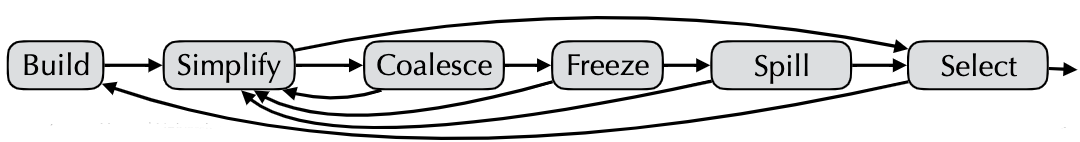
\includegraphics[width=10cm]{./img/reg_coalescing.png}
\end{figure}
\begin{figure}[htbp]
  \centering
  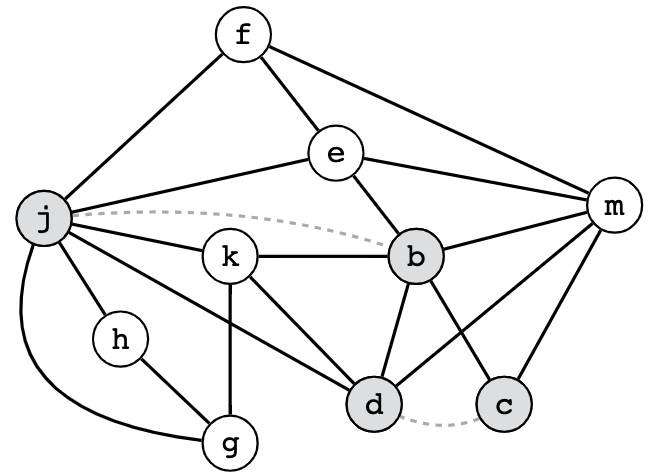
\includegraphics[width=5cm]{./img/reg_example.png}
\end{figure}
\begin{verbatim}
g:=*(j+12)
h:=k-1
f:=g * h
e :=*(j+8)
m:=(j+16)
b:=*(f+0)
c:=e+8
d:=c
k:=m+4
j:=b
\end{verbatim}
\begin{solution}

\end{solution}
\section{Coloring coalescing with pre-colored nodes\cite{cs153lec21}}
Pre-colored nodes to handle callee-save, caller-save, and special purpose registers.
\subsection{Pre-colored Temps}
\begin{enumerate}
    \item The IR often includes machine registers
\begin{enumerate}
    \item e.g., \texttt{\$fp, \$a0-\$a3, \$v0-\$v1}
    \item allows us to expose issues of calling convention over which we don't have control.
\end{enumerate}
\item We can treat the machine registers as pre-colored temps.
\begin{enumerate}
    \item Their assignment to a physical register is already determined
    \item But note that Select and Coalesce phases may put a different temp in the same physical register, as long as it doesn't interfere
\end{enumerate}
\end{enumerate}

If within a procedure:
\begin{enumerate}
    \item Move arguments from \texttt{\$a0-\$a3 (and Mem [ \$fp+offset])} into fresh temps, move results into \texttt{\$v0-\$v1}
    \item Manipulate the temps directly within the procedure body instead of the physical registers, giving the register allocation maximum freedom in assignment, and minimizing the lifetimes of pre-colored nodes
    \item  Register allocation will hopefully coalesce the argument registers with the temps, eliminating the moves
    \item Ideally, if we end up spilling a temp corresponding to an argument, we should write it back in the already reserved space on the stack...
\end{enumerate}

\subsection{Callee-Save Registers}
\begin{enumerate}
    \item Callee-Save register $r$ :
    \begin{enumerate}
        \item Is "defined" upon entry to the procedure
\item Is "used" upon exit from the procedure.
    \end{enumerate}
\item Trick: move it into a fresh temp
\begin{enumerate}
    \item Ideally, the temp will be coalesced with the calleesaves register (getting rid of the move)
    \item Otherwise, we have the freedom to spill the temp.
\end{enumerate}
\end{enumerate}
\subsection{Caller-Save Registers}
\begin{enumerate}
    \item Want to assign a temp to a caller-save register only when it’s not live across a function call  
    \begin{enumerate}
        \item   Since then we have to save/restore it 
    
    \end{enumerate}
       \item So treat a function call as “defining” all caller-save registers.
\begin{enumerate}
    \item Callee might move values into them 
    \item Now any temps that are live across the call will interfere, and register assignment will find different registers to assign the temps.
\end{enumerate}

\end{enumerate}

\subsection{Compile the following C function }
\begin{enumerate}
    \item Assume target machine has 3 registers
    \item \texttt{\$r1} and \texttt{\$r2} are caller-save
    \item \texttt{\$r3} is callee-save
\end{enumerate}
\begin{minted}[mathescape,linenos]{c}
int f(int a, int b) { 
  int d = 0; 
  int e = a; 
  do {  d = d+b; e = e-1; } 
  while (e > 0); 
  return d;
}
\end{minted}
\begin{verbatim}
f: c := $r3 ;preserve callee;
a := $r1 ;move arg1 into a;
b := $r2 ;move arg2 into b;
d := 0
e := a
loop: 
 d := d + b 
 e := e - 1 
 if e > 0 loop else end
end: 
 r1 := d ;return d;
 r3 := c ;restore callee;
 return ;$r3,$r1 live out 
\end{verbatim}
\begin{figure}[htbp]
  \centering
  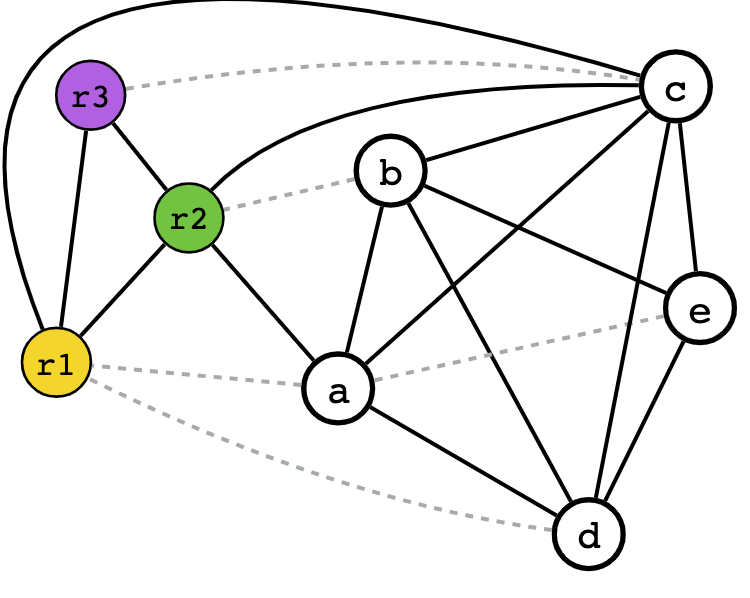
\includegraphics[width=5cm]{./img/reg_example2.png}
\end{figure}
\begin{solution}

\end{solution}
\printbibliography

\end{document}
